\chapter{Animation}
\label{chapter2}

The animatable body exported by Blender is in Ogre xml mesh and skeleton format. They are converted to binary skeleton and mesh files by the OgreXML serializer, and imported natively into the software. Prior to animation, the bones are initialized to be oriented by the data from depth sensor. Afterwards, they are updated with the orientation data.

\section{Initialization}
\label{section2_1}

Animatable meshes are loaded and maintained via the SkeletalMesh class I have implemented, which bridges the gap between Ogre�s skeletal animating system and the input from Kinect sensor. When an instance of the object is initialized, it is given a mesh file. After the mesh is loaded with the skeleton data, the bone list is iterated through, given the initial orientation uniquely for each animatable bone with the Kinect sensor. 

The animatable bones are set to be manually controlled, not inherit orientation from parents, given the initial orientations. At that state, the bone is set to initial state, to be reset at every frame with updated orientations. The non-animated bones are left to be automatically controlled and inherit orientation in order to keep them aligned with their parent bones. 

\section{Animation}
\label{section2_2}
Every frame, the orientation information from the bones are extracted in 3x3 matrix form., along with the confidence of the sensor in that orientation. If the confidence is less than 0.5 in 1, the bones are left as they were in the previous frame to avoid unnatural movements. 

The matrix from the Kinect is row major, whereas Ogre works with column major matrices. The transpose matrix is given to Ogre, turned into a quaternion and converted to local coordinate space. The updated orientation is fed into the bone, after it is multiplied with the initial orientation. The root bone is translated in local space in the end, to simulate the translation, above rotation.

This technique is used with the top-part of the dress as well, and it will be used for jackets, shirts and other clothing ware which do not leave the body surface by a great distance. 


\section{Motion Filtering}
\label{section2_3}

Application of the raw data from the sensor causes unnatural movements due to the noise in the sensor input, self-occlusions of the body and inadequate IK solvers.  In order to present a more realistic avatar animation, a series of filters and constraints are applied to the sensor data. 

\subsection{Position Filtering}
The most severe disruption of the self-occlusion problem takes place in the joint position acquisition. There is no possible way of acquiring the correct position of a limb when the sensor has no vision of it. However, the way humans move their limbs under normal conditions follow certain principles and trends, which can be used to estimate the locations of occluded body parts. The nature of these motions, demonstrating traits similar to seasonal behavior, makes them suitable for applying a variety of filters~\cite{Azimi2012}. We decided to go with the Holt-Winters double exponential smoothing~\cite{Holt2004,Kalekar2004} as it comes with the middleware, easy to use and delivers good quality results with acceptable latency for the purposes of this application. 

\subsection{Rotation Filtering and Constraints}
The joint orientations are acquired from the sensor middleware directly, however the data is not smooth. Although the middleware enforces certain constraints (such as allowing only pitch rotations on ulna), there are often significant gaps in the estimated angles that produce unnatural tremor-like movements on the avatar. Furthermore, there is no filtering of unnatural rotations that take place when an occluded body part is estimated to be in a wrong location. 

The inferior quality of the orientation data is improved in two stages: applying another set of constraints on the joint data based on the natural limits of human bones, followed by an asymptotic smoothing of the joint angles to prevent the effect of gaps in the angles (see~Figure~\ref{fig:rotation-filter}). 

\begin{figure}[htbp]
	\centerline{ 
	\fbox{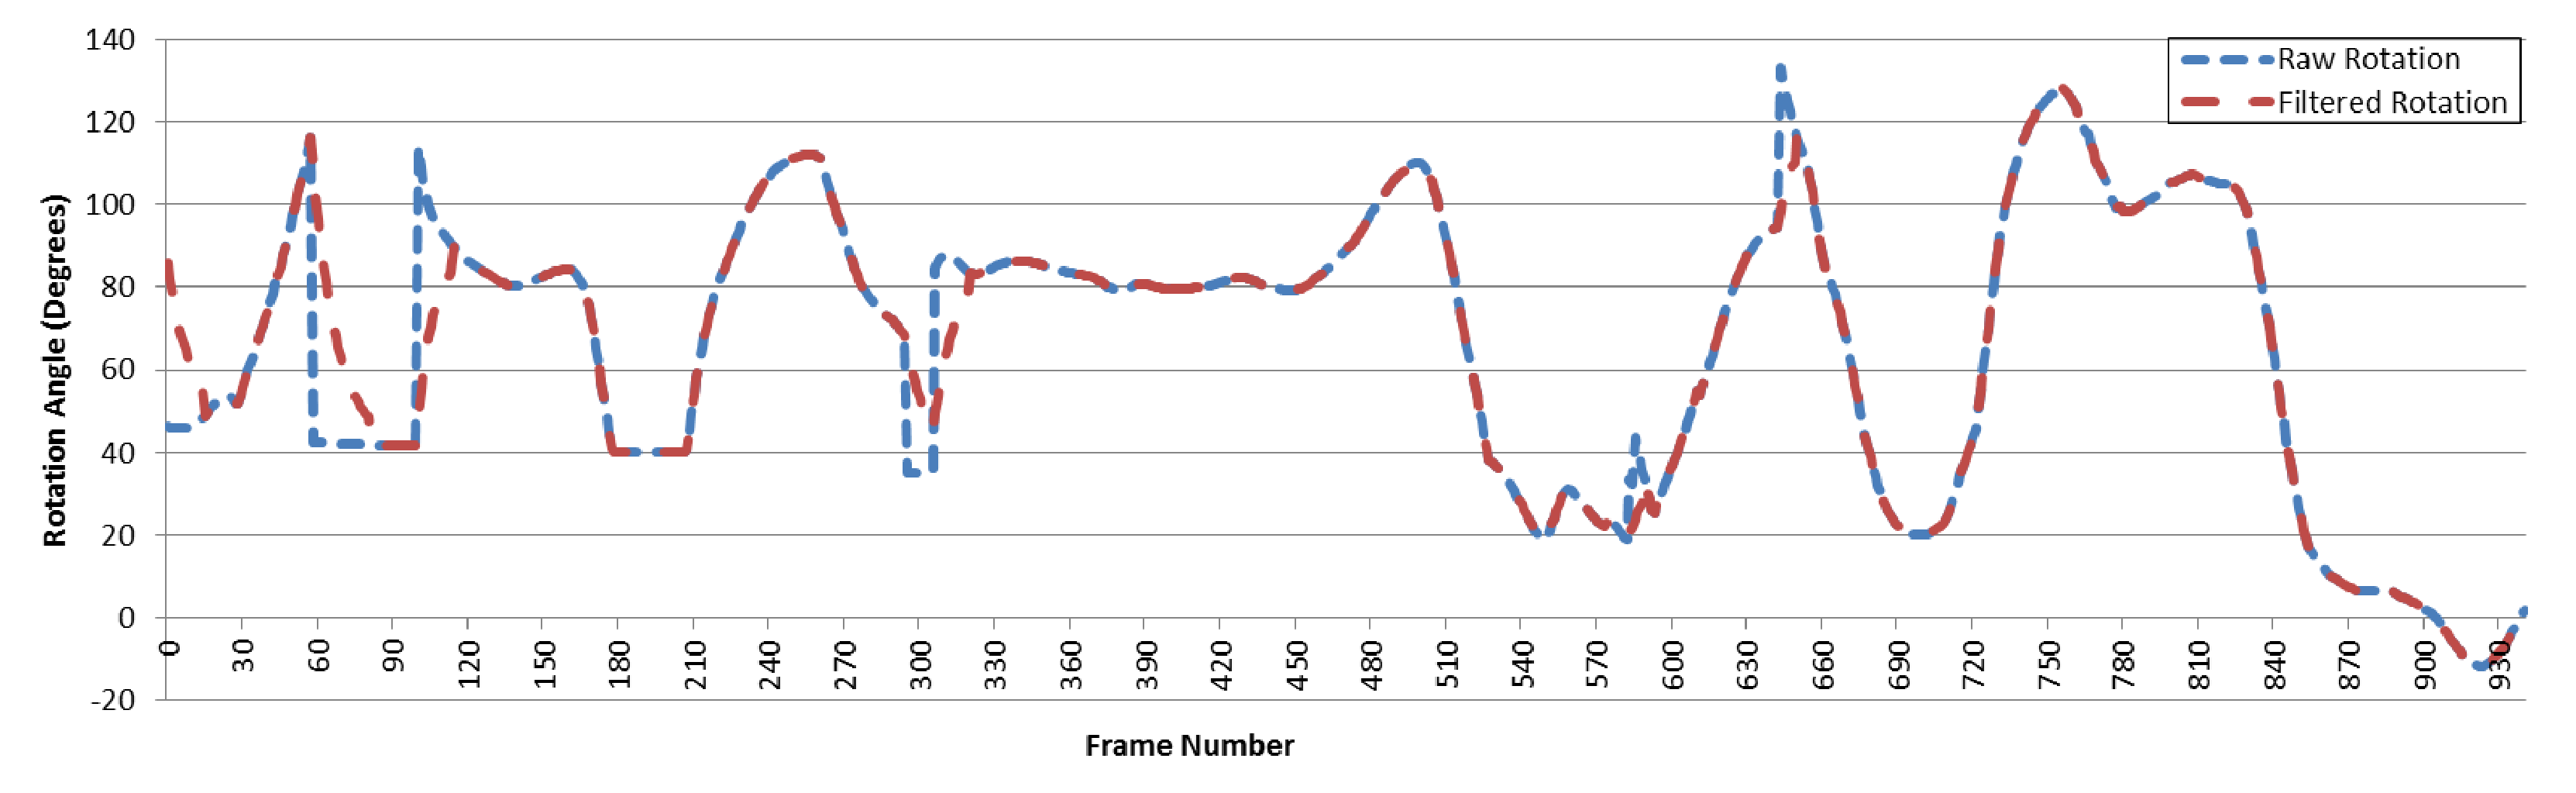
\includegraphics[width=0.98\textwidth]{./figures/rotation-filter.eps}}
	}
\centerline{\ }
\caption{The row and filtered samples for right the humerus roll angle}
	\label{fig:rotation-filter}
\end{figure}


\subsection {Bone Splitting}
The lower sections of human limbs contain two parallel bones allowing the twisting rotation on the hands and feet. The configurations of bones allow all portions of the lower limbs follow the bones in pitch and roll rotations, although the effect of yaw rotation decreases as it gets closer to the mid-section joint (elbow or knee). This effect is not possible to achieve with a single bone fore-arm representation, as specified in the highest level of detail in the H-ANIM standard~\cite{HANIM}, using unified weights (same for all types of rotations, transformations and scaling) and linear skinning. On the other hand, applying a different set of weights for each possible transformation, rotation or scaling requires additional space and time, which can be considered redundant because it is not going to be used in most parts of the skeleton and surface mesh; thus, it is not implemented in most of the popular rendering engines. This problem is addressed by Kavan et al.~\cite{Kavan2009}, proposing a method of introducing additional blending bones to simulate non-linear skinning. However, this approach is not suitable for a real-time application with previously unknown motions. 

Because our only problematic bones for this particular case is the upper limbs, we employed a novel approach to solve this problem by introducing an additional bone connected in series for the upper limbs. The humerus and ulna bones are split halfway and the lower sections are labeled as humerus-extension and ulna-extension, respectively. The vertex weights in the corresponding sections are divided linearly among two sections, as seen in Figure~\ref{fig:forearm-weights}. 


\begin{figure}[htbp]
	\centerline{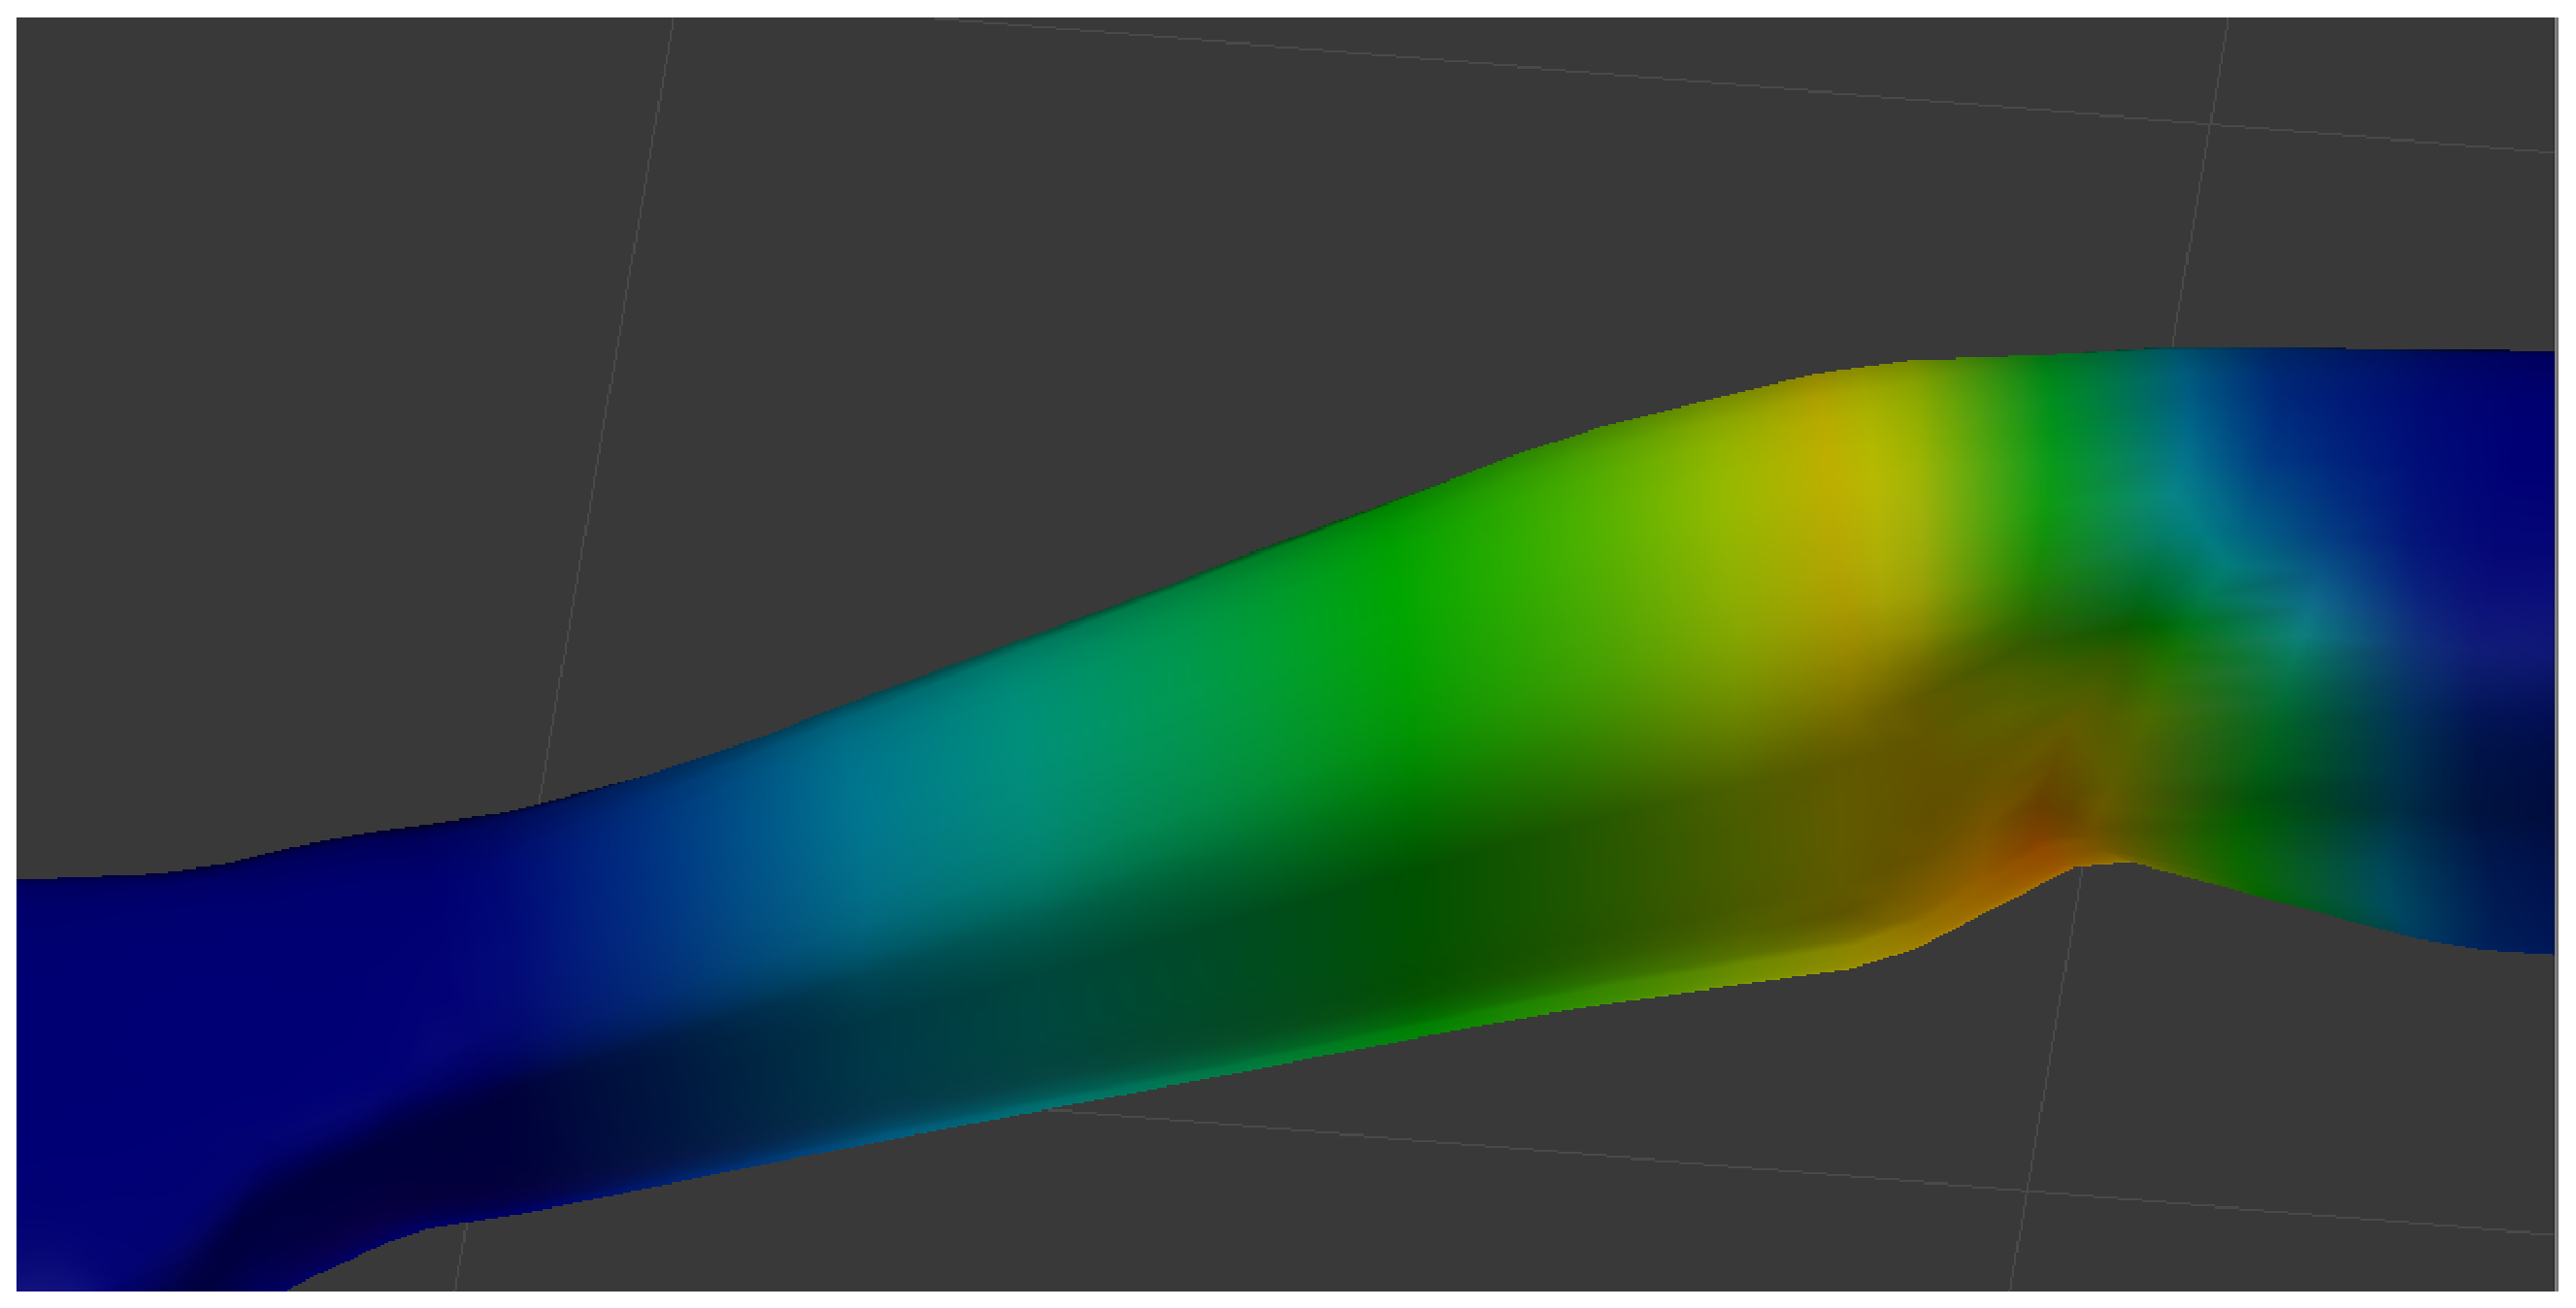
\includegraphics[width=0.75\textwidth]{./figures/ulna-weight.eps}}
	\centerline{(a)}
	\centerline{\ }
	\centerline{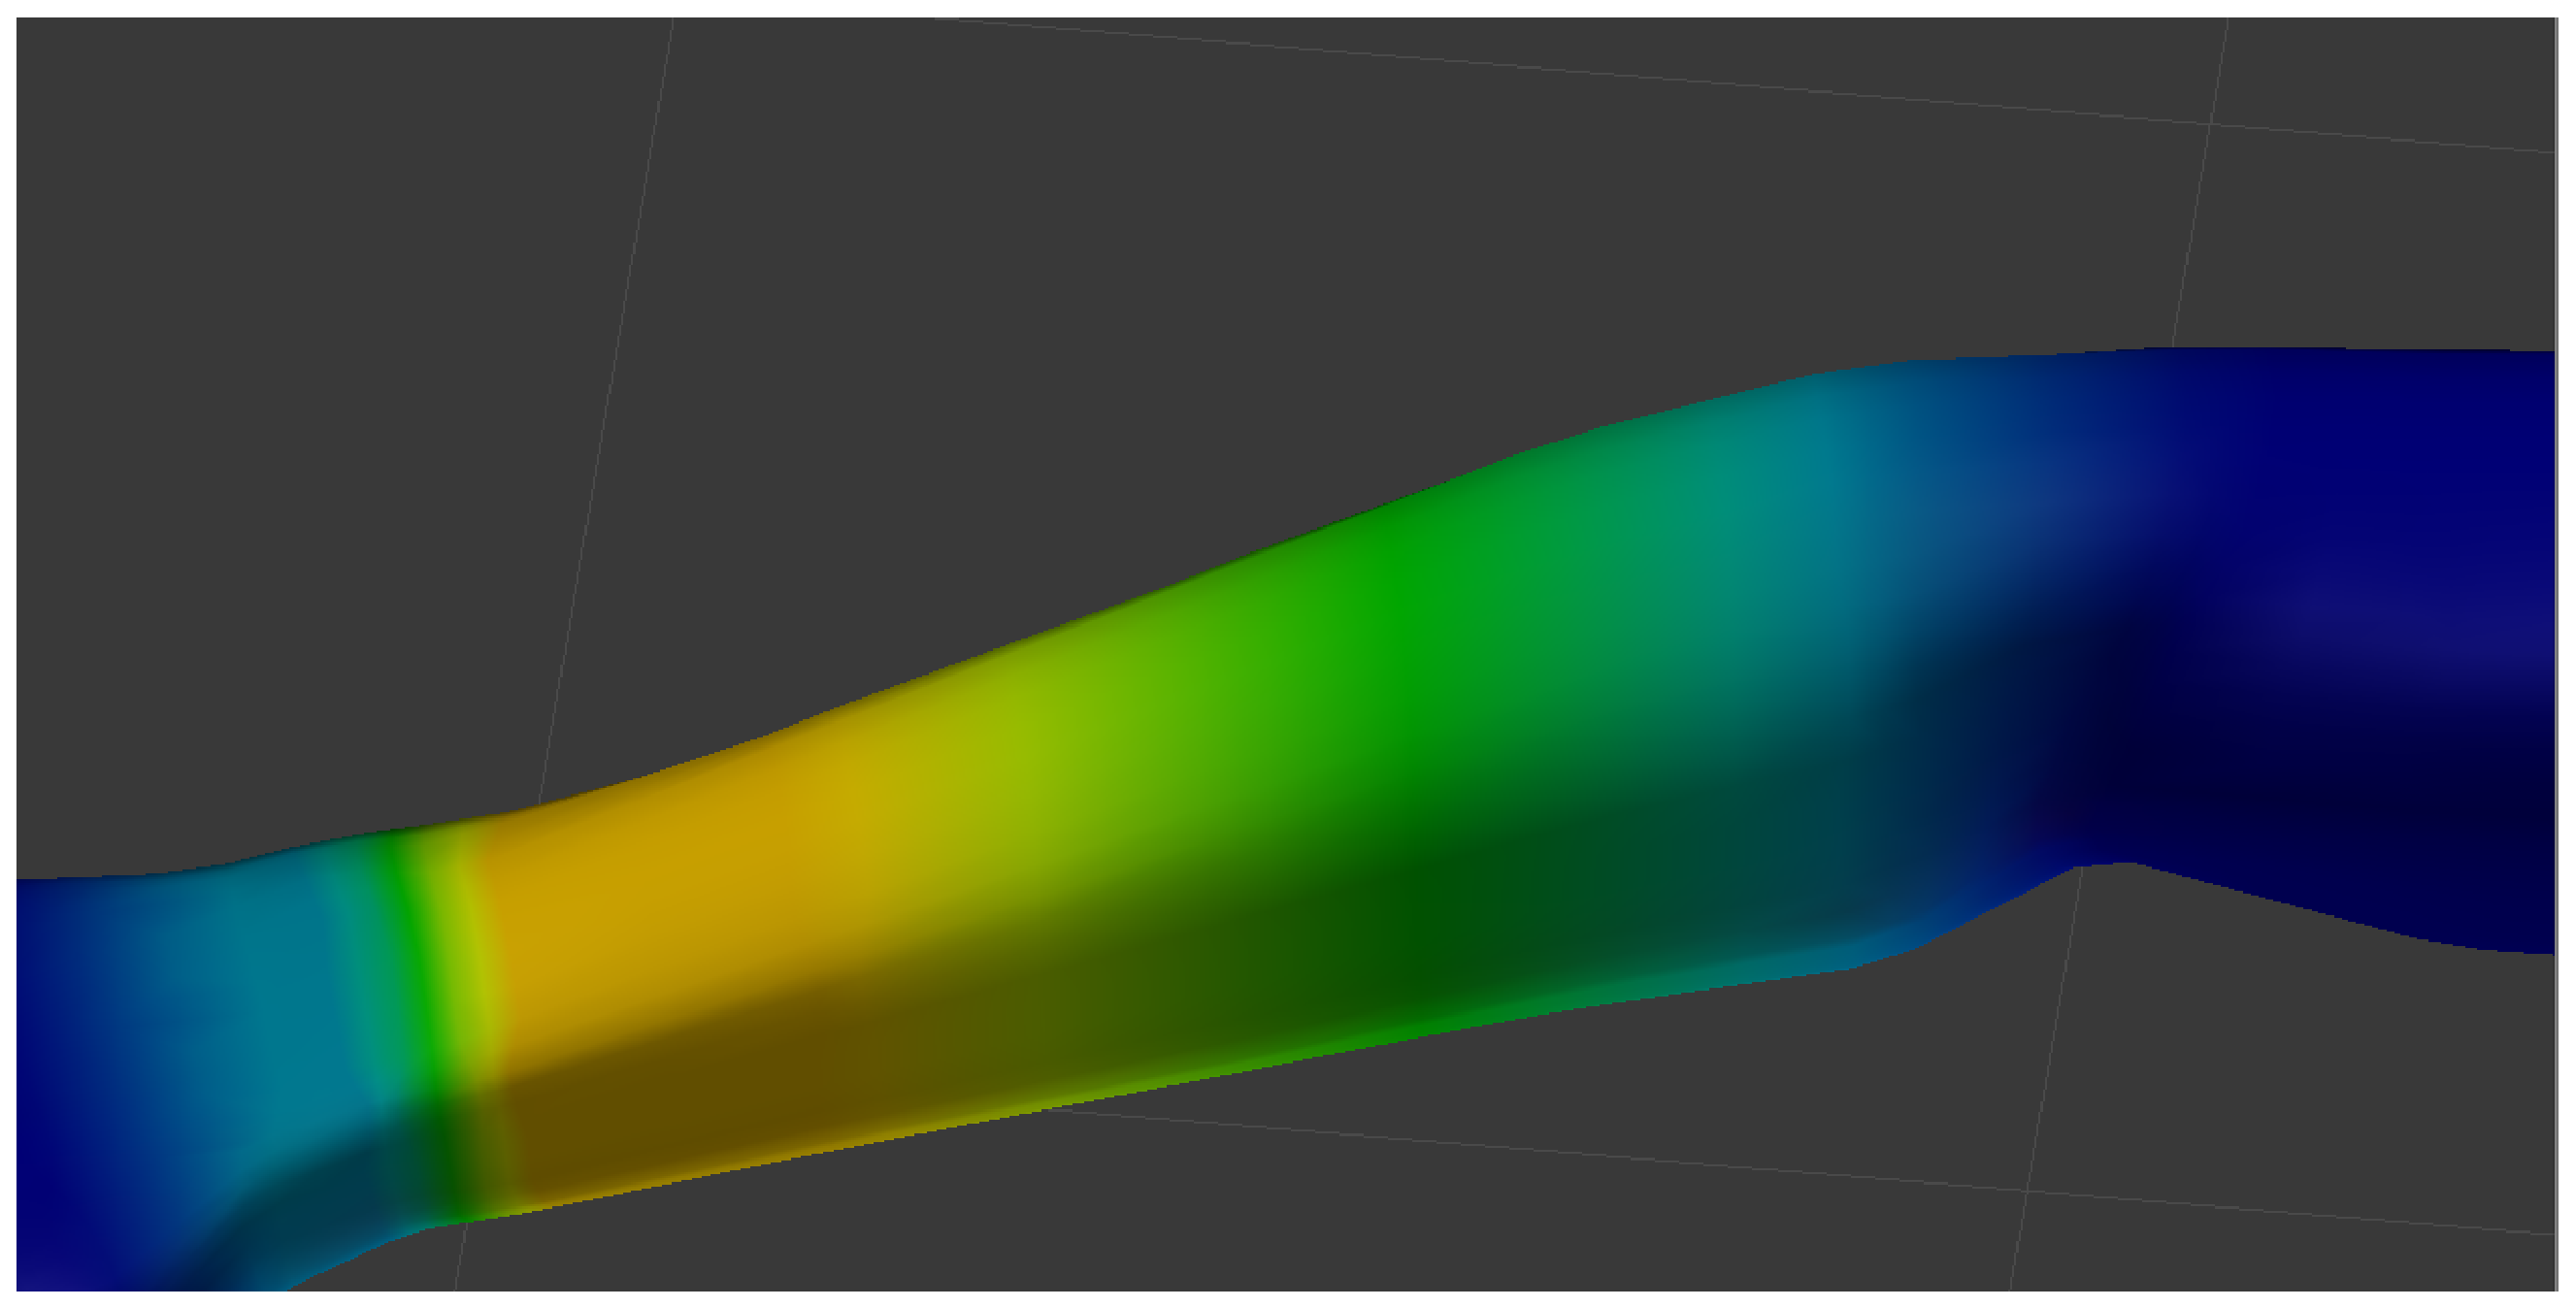
\includegraphics[width=0.75\textwidth]{./figures/ulna-extent-weight.eps}}
	\centerline{(b)} 
	\centerline{\ } 
	\caption{The vertex weights for (a) the upper ulna and (b) the lower ulna bone (weight increases from blue to yellow).}
	\label{fig:forearm-weights}
\end{figure}

During runtime, the filtered local rotation of the upper limb bones are separated into two distinct rotations, one containing the yaw and the other containing pitch and roll rotations, which are applied to the extension bone and the original bone, respectively. With proper weights, the rotation of the users arm is transferred to the virtual avatar naturally without introducing any artifacts. As seen in Figure~\ref{fig:forearm-comparison}, the vertices on the forearm twist in a more natural way resembling the real motion.

\begin{figure}[htbp]
	\centerline{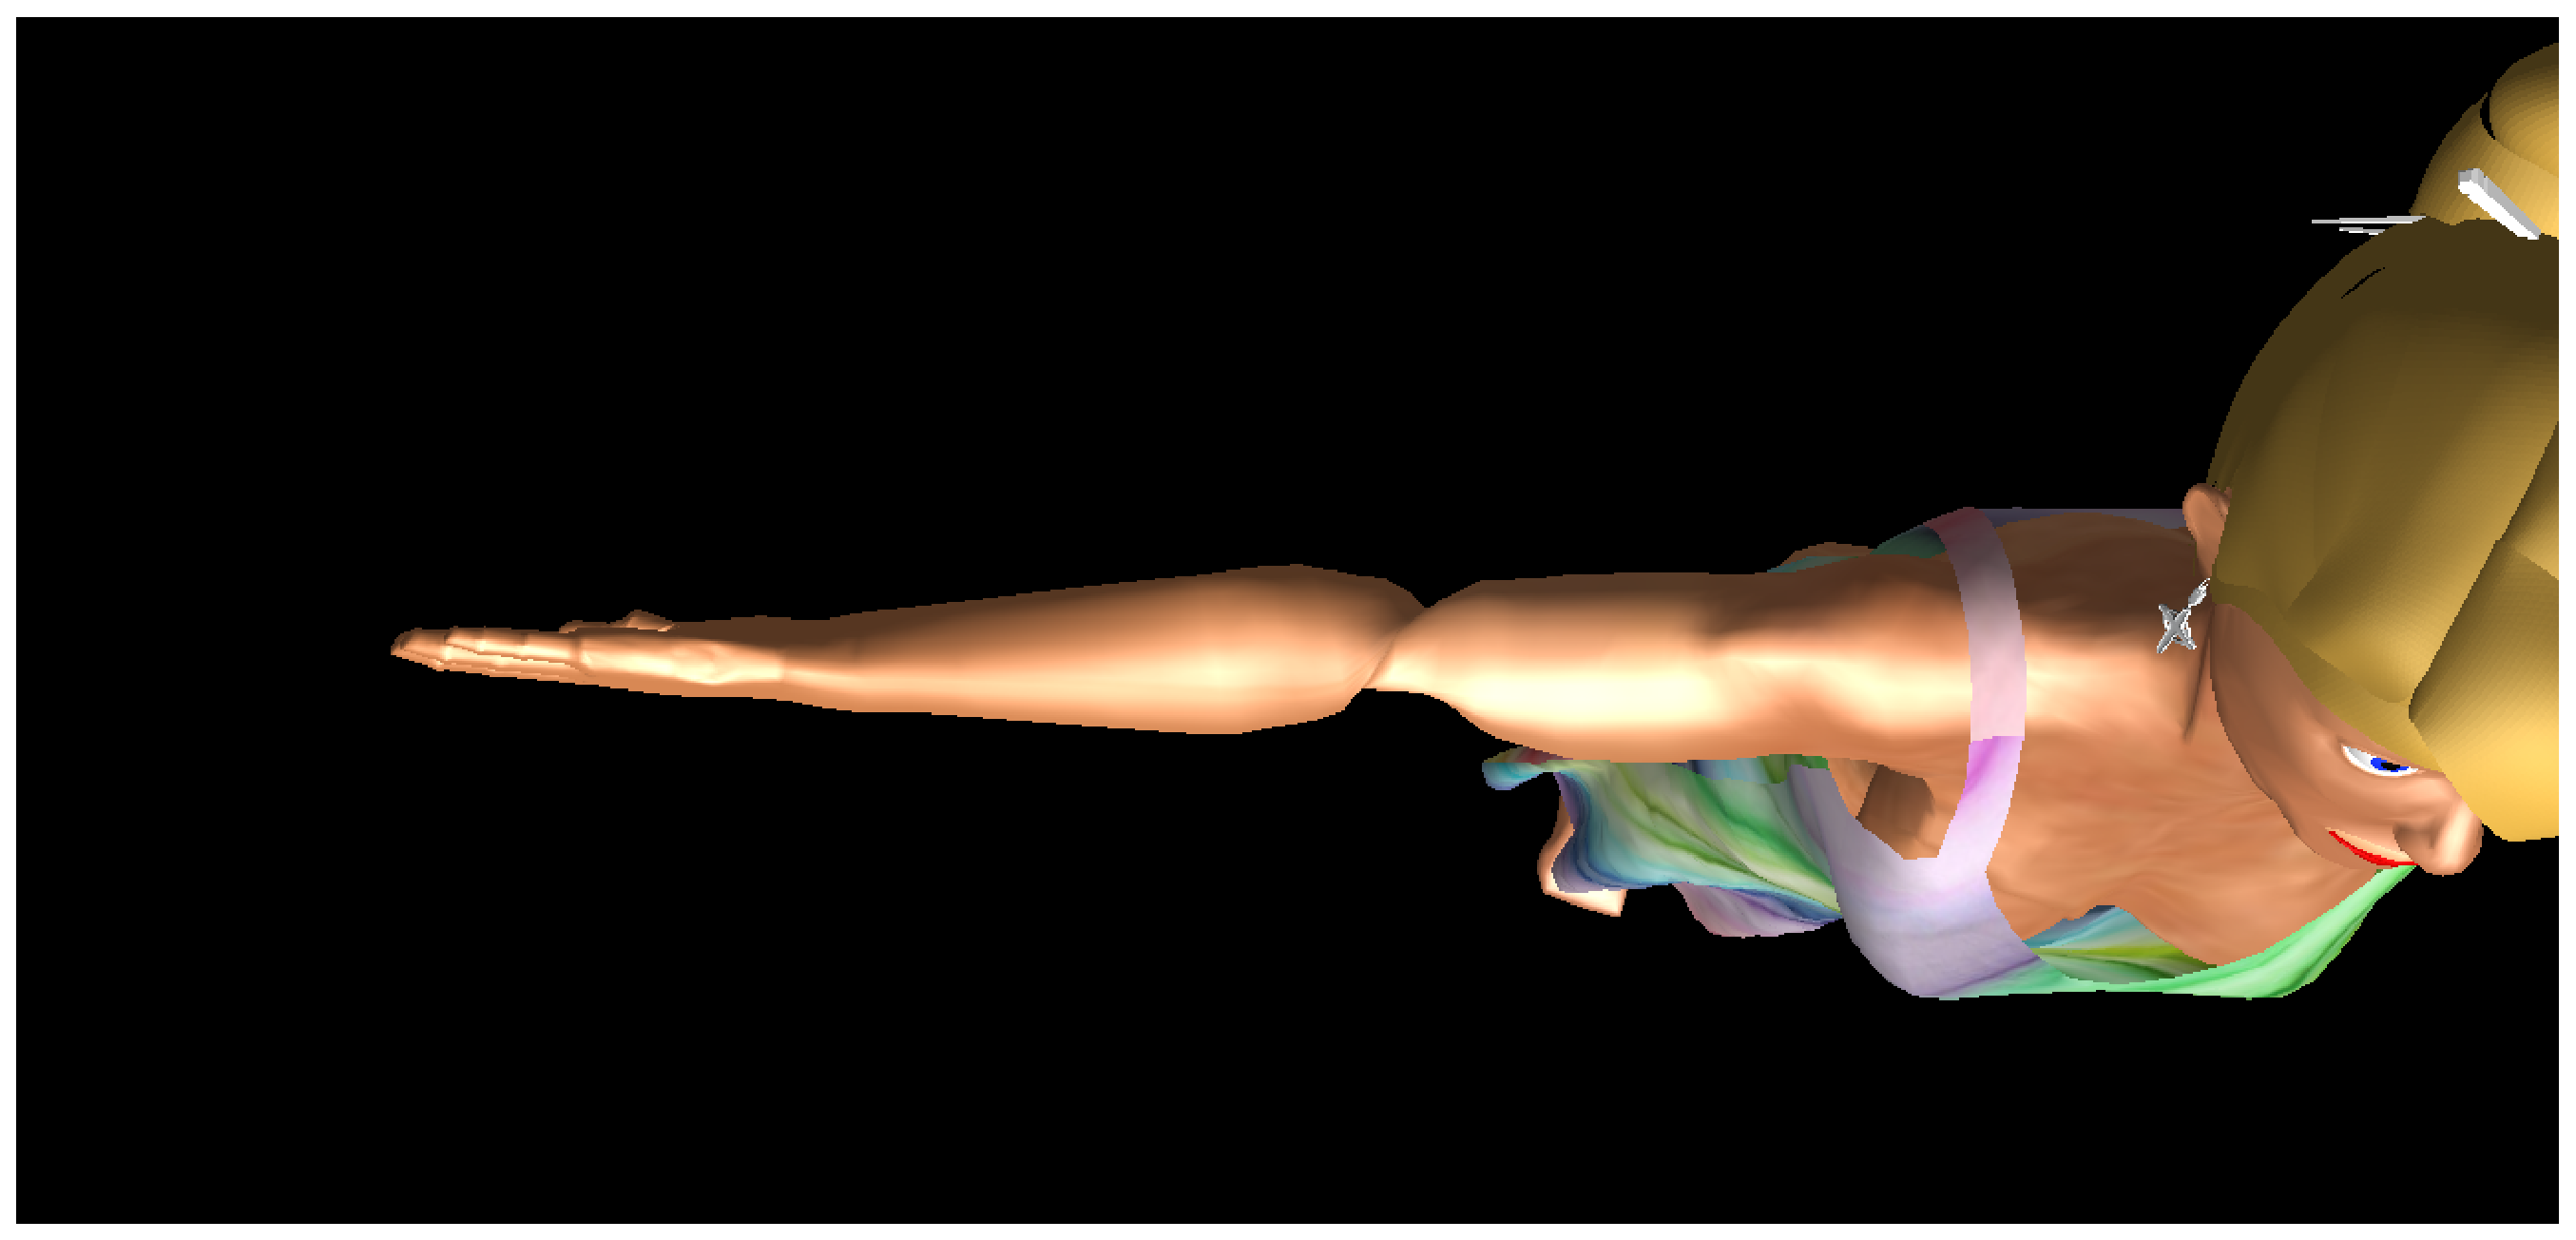
\includegraphics[width=1.0\columnwidth]{./figures/fore-arm-single-bone.eps}}
	\centerline{(a)}
	\centerline{\ }
	\centerline{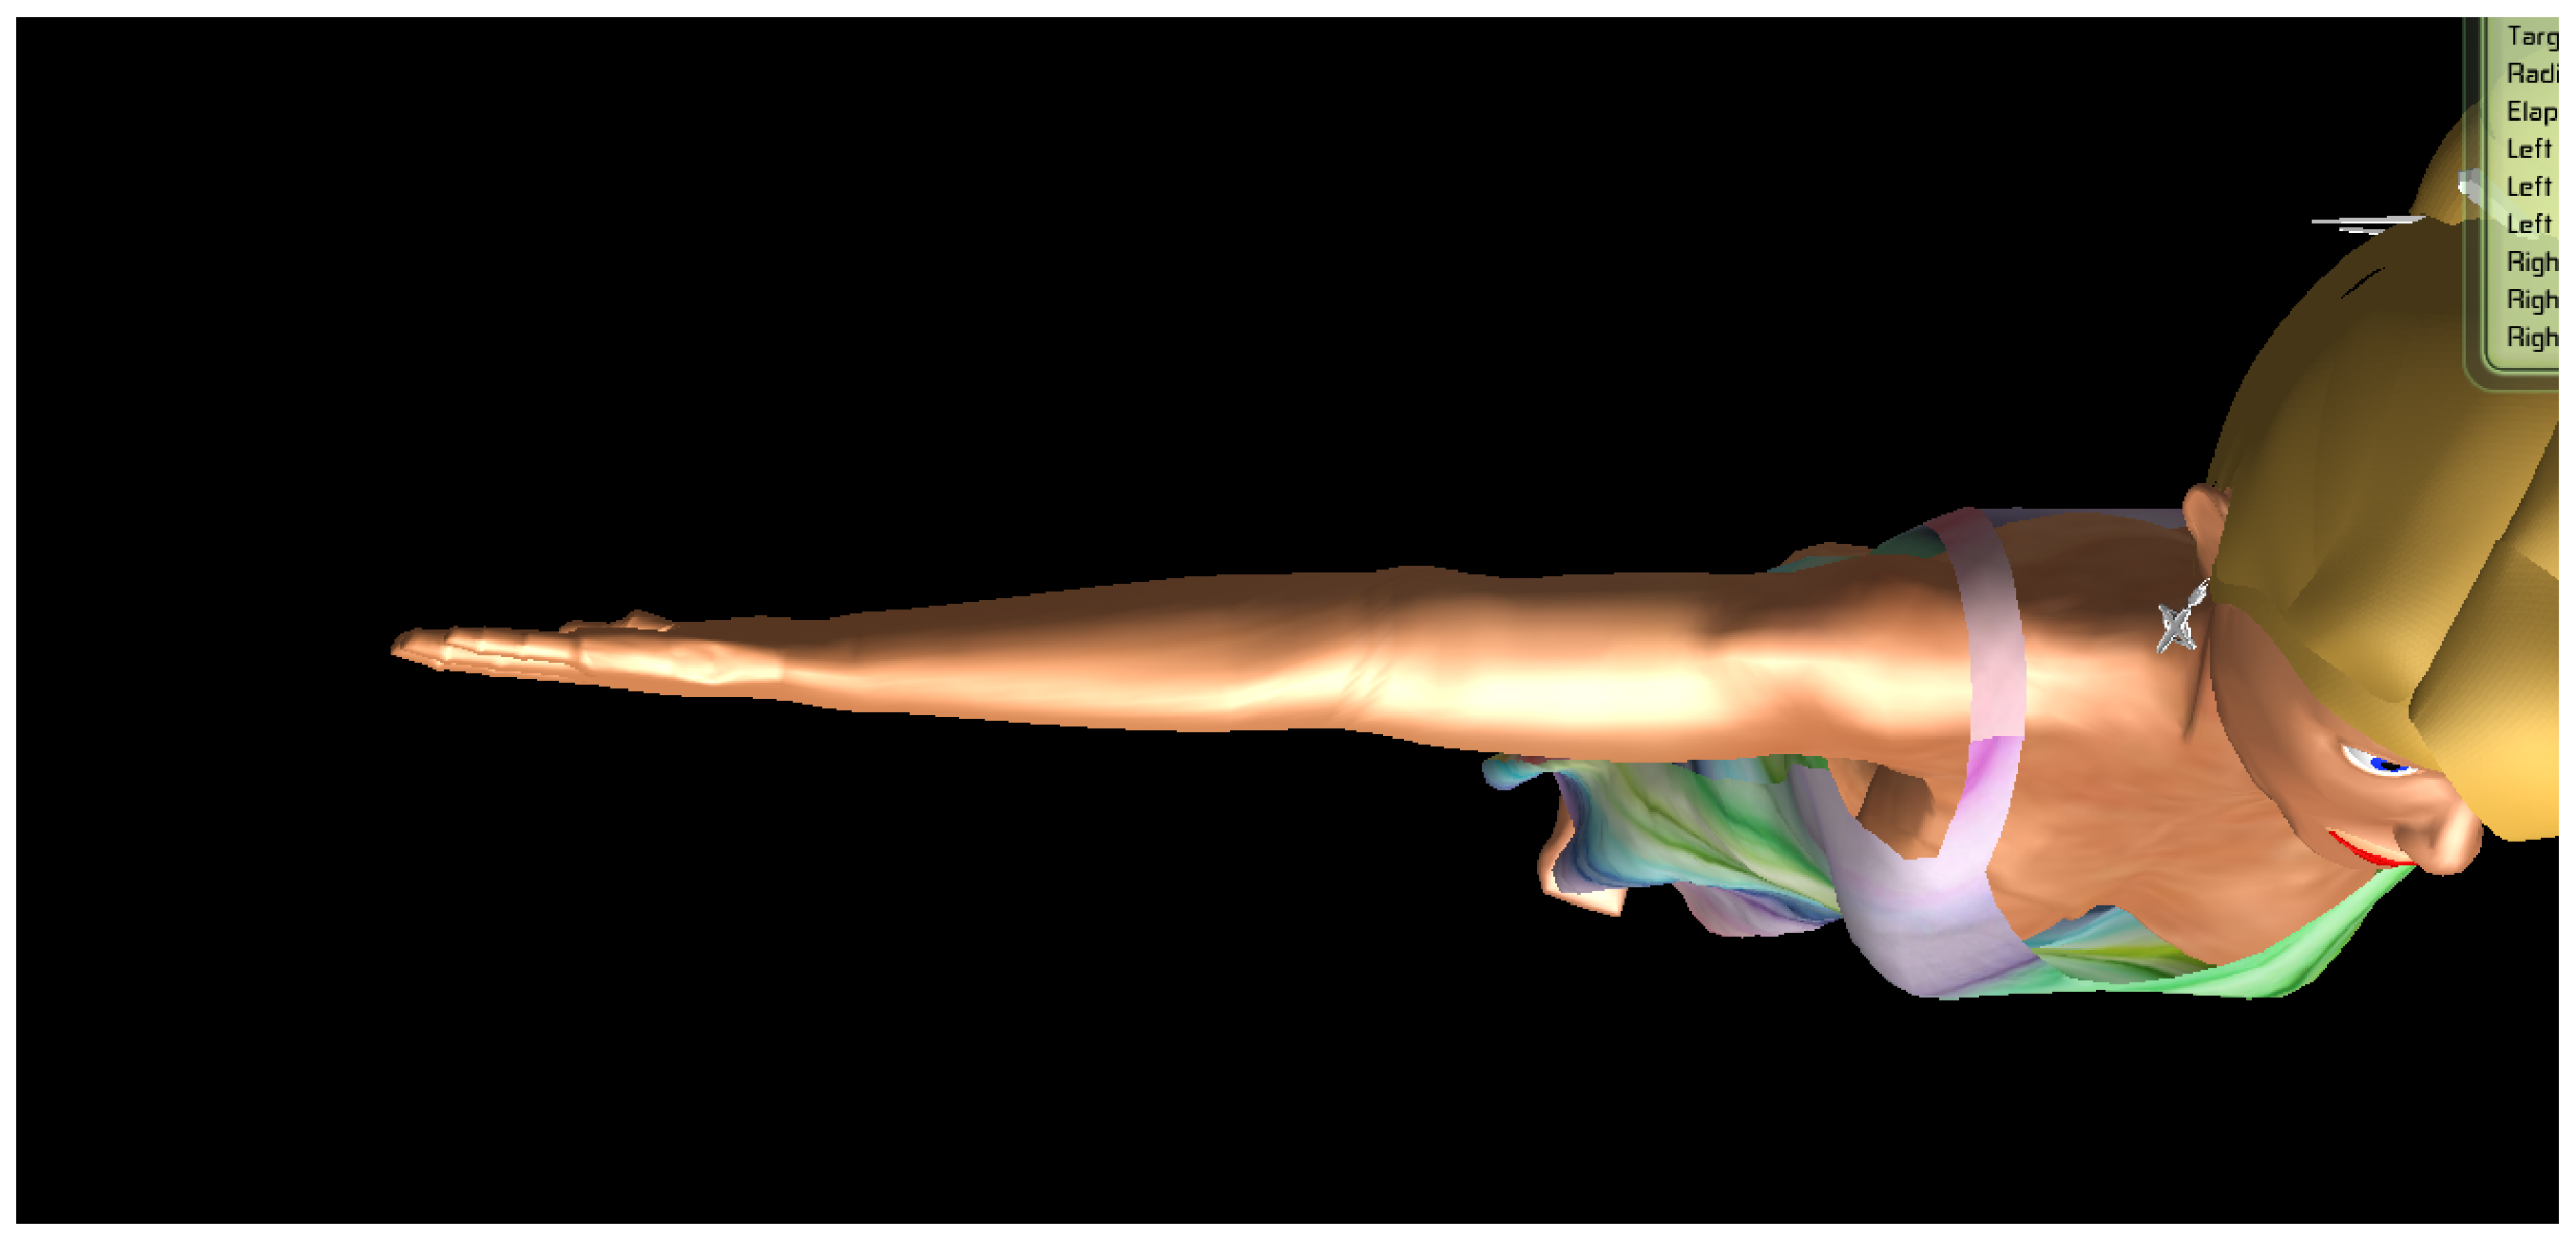
\includegraphics[width=1.0\columnwidth]{./figures/fore-arm-double-bone.eps}}
	\centerline{(b)}
	\caption{Comparison of a -90$^\circ$ yaw rotation on the forearm with: (a) single and (b)~double-boned skinning.}
	\label{fig:forearm-comparison}
\end{figure}

\section{Algorithm}
\label{section2_5}

I used linear weighted skin blending \cite{Kavan2003} in order to simulate deformation on the characters skin. The effects of four bones with different weights are combined linearly to change the positions and normal of vertices.

\subsection{The bone transformation Pseudo Code}

The pseudo code below is executed during the pre-render cycle. The bone
orientations are set to be ready for animation, deformation and rendering. At
every render cycle, update Skeleton function is called, which automatically
fetches the coordinates from the Kinect and sets up the skeleton for vertex
blending. 

\begin{algorithm}
\dontprintsemicolon % Some LaTeX compilers require you to use \dontprintsemicolon instead
\SetKwBlock{function}{function}{endfunction}
\function(transformBone\ArgSty{(bone)}){
\KwIn{A bone and the corresponding orientation matrix from Kinect}
\KwOut{The same bone with updated orientation}
$q_I =$ initial orientation of bone\;
$q_N =$ relative orientation\;
$q_K = 3\times3$ Orientation Matrix From Kinect\;
\If{$kinect_{confidence} > 0.5$} {
  $q_Q = toQuaternion(q_K)$\;
  $q_N = toLocalSpace(q_Q)$\;
  $q = q_N \times q_I$\;
  $bone.orientation=q.normalise{\left(\right)}$\; }}

\If{$user$ ${\bf is }$ $new$} {
  $p_{torso}.initialize()$\tcc*{Initialize torso position}  \;
 }
\ForEach {bone}{
\If{$bone_{orientation}$ ${\bf is }$ $new$}{
$transformBone(bone)$\;
$skeleton.needsUpdate()$\;}}
\caption{Bone transformation algorithm}
\label{algo:transformBone}
\end{algorithm}

\subsection{Deformation Pseudo Code}

Algorithm \ref{algo:updateMesh} is executed prior to rendering, to update the
vertices of the skin. The vertex blending function is where the deformation
actually occurs.

\begin{algorithm}
\dontprintsemicolon % Some LaTeX compilers require you to use \dontprintsemicolon instead
\SetKwBlock{function}{function}{endfunction}
\function(prepareBlendMatrices\ArgSty{(mesh)}){
\ForEach {bone}{
bone.applyScale()\;
bone.applyTransform()\;
bone.applyOrientation()\;
}
$i=0$\;
\ForEach {bone}{
$m[i] = bone.getTransformationMatrix4\times4$\;
$i++$\;
}
mapIndex=mesh.getIndexMap() \tcc*{Index Map contains the bone pointers for
every vertex}\;
$i=0$\;
\ForEach {indexSet ${\bf in }$ mapIndex}{
$m_b[i] = indexSet[i]+m$ \tcc*{Blend matrices are pointers to the individual
bone matrices}\;
$i++$\; }
\Return $m_b$\;
}

\function(vertexBlend\ArgSty{($m_b$)}){
pos=*mesh.positions\tcc*{Pointer to the position matrix}\;
norm=*mesh.normals\tcc*{Pointer to the normal matrix}\;
$b_i=$*mesh.blendIndices\tcc*{Pointer to the blend index matrix}\;
$b_w=$*mesh.blendWeights\tcc*{Pointer to the blend weight matrix}\;
\ForEach {4 vertices ${\bf in }$ pos}{
\ForEach {vertex ${\bf in }$ 4 vertices}{ 
$m[1,2,3,4]=m_b[b_i[vertex]]$ \tcc*{Weighting Bones}\;
$m_c[j]=collapseMatrix(m,b_w[vertex]){\bf (i)}$\;
}
$pos[4 vertex]=m_c\times pos[4 vertex]$
$norm[4 vertex]=m_c\times norm[4 vertex]$
}}
\If {skeleton needs update}{
$m_b=prepareBlendMatrices(skeleton.mesh)$\;
$vertexBlend(m_b)$\;
}
\caption{Mesh update algorithm called at every frame.}
\label{algo:updateMesh}
\end{algorithm}

{\bf (i)}:In my models, every vertex is assigned to at most 4 different bones.
In order to speed up the deformation process, the transformation matrices for the corresponding matrices are collapsed into one. Collapsing is simply weighted addition of the four weighting matrices for a vertex.

\subsubsection{Matrix Operations}
After four sets of matrix for four vertices are collapsed into four matrices, the following matrix operations are performed. 4 vertices are processed together in order to fully utilize the matrix multiplication features.
Let us take the weighted matrix for vertex i:

\begin{equation}
M_i=
\begin{bmatrix}
m_{00}^i & m_{01}^i & m_{02}^i & m_{03}^i \\
m_{10}^i & m_{11}^i & m_{12}^i & m_{13}^i \\
m_{20}^i & m_{21}^i & m_{22}^i & m_{23}^i \\
0 & 0 & 0 & 1
\end{bmatrix}
\label{eqn:weighted_matrix_for_i}
\end{equation}

Note that this matrix is a linear combination of four linear
transformation matrices from four weighting bones, hence the $3^{rd}$ row is by
default  [0 0 0 1].

We also have the initial positions for the 4 vertices as $[p^i_x \: p^i_y  \:
p^i_z  \: 1]$.$3^{rd}$ value, which is one is not included in the vertex buffer
and it will not be taken into account with the calculations.

In order to generate an efficient SIMD process, I will perform 4x3 dot product
calculations in each instruction. Dot products are commanded in the machine language, which makes it more preferable to higher level matrix calculations. To acquire the simulated x coordinates for the four vertices, we combine the first rows of all collapsed matrices for all and transpose it:

\begin{equation}
M_T=
\begin{bmatrix}
m_{00}^0 & m_{00}^1 & m_{00}^2 & m_{00}^3 \\
m_{01}^0 & m_{01}^1 & m_{01}^2 & m_{01}^3 \\
m_{02}^0 & m_{02}^1 & m_{02}^2 & m_{02}^3 \\
m_{03}^0 & m_{03}^1 & m_{03}^2 & m_{03}^3 
\end{bmatrix}
\label{eqn:transposed_weight_matrix}
\end{equation}

To coincide with the transposed matrix, I also create a position matrix with positions from all vertices:

\begin{equation}
P_T=
\begin{bmatrix}
p_{x}^0 & p_{x}^1 & p_{x}^2 & p_{x}^3 \\
p_{y}^0 & p_{y}^1 & p_{y}^2 & p_{y}^3 \\
p_{z}^0 & p_{z}^1 & p_{z}^2 & p_{z}^3  
\end{bmatrix}
\label{eqn:transposed_weight_matrix}
\end{equation}

Next, the matrices $M_T$ and $P_T$ are multiplied in a row-by-row fashion and
summed together:

\begin{equation}
d_x=M_{T0} \times P_{T0} + M_{T1} \times P_{T1} M_{T2} \times P_{T2} +M_{T3}
\label{eqn:transposed_weight_matrix}
\end{equation}

The result vector $d_x$ is a 4x1 vector which has the post-blended vertex
x-coordinates: $[P^0_x \: P^1_x  \: P^2_x  \: P^3_x]$. The same procedure is
applied to the normal of a vertex. Process continues with the next set of four vertices.

\section{Interaction Between the Body And Cloth}
\label{section2_4}
The movements of the user are passed on the pieces of cloth separately.

\subsection{Non-Simulated Section}
Non simulated parts of the clothes are the ones which do not get separated from
the body most of the time. Most parts of our clothes usually stick to the body and experience the same deformation as our skin. In order to increase performance, detailed simulation on these parts are not run, instead they are deformed the same as the remained of human body. In the full-body dress I am working with, the part above the waist has a skeleton similar to the body and the information from the Kinect is passed on to this portion as well. It is treated as a part of the actual avatar.

\subsection{Simulated Section}
The movements of the body are transferred into the simulated section of the cloth in three main ways:

\subsubsection{Transformation}
The fixed vertices are transformed to match the remainder of the cloth. The
transformation is done on the rendering level, the physx world experiences no difference in transformation manner. This process keeps the cloth aligned with the rest of the visible world.

\subsubsection{Collision}
The colliding body is updated and collided with the cloth. The colliding body
consists of 16 spheres and the capsules connecting the spheres. The details of
this body is explained in section \ref{section_4_1}. This process keeps the
cloth out of the avatar’s way.

\subsubsection{Inertia}
The Inertia of transformations is passed onto the simulated cloth, increasing
the realism. The passed on inertia comes from the rotation and the transformation of the root bone of the human skeleton. With this process, although there is no actual transformation in the physics world, the resulting inertia effects are visible on the cloth itself. 

\section{Handling Foot Skating Problem}
\label{section2_5}
The virtual model is aniamted by changing bone orientations and root bone position. If the orientations and root position are applied to 
the bones respecively, the feet of the character appear to be floating on the ground which deteriorates the realism of the system. 

This issue, known as footskating is not limited to depth sensor applications. It has been detected in motion capture systems and solved sufficiently with approaches by 
Kovar et al.\cite{Kovar2002} and Ikemoto et al.\cite{Ikemoto2006}. However, the proposed methods in these approaches rely on some sort of preprocessing or supervised learning,
which is not suitable for our system, as the motion is captured and applied im real time. Hence, a solution which does not require a training process is needed for such applications. 
Mankyu and Choi \cite{Mankyu2013} proposed a similar method which does not require training for real-time depth sensor applications. 

I adapted Mankyu's and Choi's approach to overcome the footskating problem in my framework. However it required additional filters and constraints in order to be usable in extended 
animations. It is assumed that one of the feet is always on the ground, artifacts may occur if the user attempts jumping. The whole footskating algorithm consists of 5 steps. 

\begin{enumerate}
\item Determine which foot is constrained by checking speed and location thresholds. The thresholds are changed adaptively in order to compensate for different sensor and user placements.
\item Place the constrained foot at its last recorded position and solve the inverse kinematics problem to determine the orientations of the hip and knee joints. Solving an inverse kinematic
problem is no trivial task. There are various numerical and analytical methods for inverse kinematic problems and many implementations focusing on each. For our framework, we embedded 
the IKAN library by Pennsylvenia University \cite{IKAN2013}, which uses the approach by Tolani et al.\cite{Tolani2000}.  
\item Check if the foot coincides with its intended position after the inverse kinematic orientations are applied to the bones. If there is a positional mismatch, relocate the root joint to complete alignment.
\item Smooth the joint orientation difference in order to avoid jumps from frame to frame. This is especially important when the constraint switches, as the source of the orientations are different in two cases and they do not always overlap. 
\end{enumerate}

The overall algorithm consists of two major parts: constraint checking and adaptation (in Algorithm \ref{algo:check_foot_constraints}) and joint angle determination and application (in Algorith \ref{algo:foot_skating}).  

\begin{algorithm}
\dontprintsemicolon % Some LaTeX compilers require you to use \dontprintsemicolon instead
\If{$isFirstFrame$}{
\If{$p^y_{left} < p^y_{right}$ }{
	$constrained = left$\;
	$y_{threshold}=p^y_{left}$\;
}
\Else {
	$constrained = right$\;
	$y_{threshold}=p^y_{right}$\;
}
}

\If{$constrained is left$}{
	\tcc{Check if constraints still hold}
	\If{$p^y_{left} > y_{threshold} and v_{left} > v_threshold$}{
		\tcc{Foot is not constrained anymore, check other foot}
		\If{$p^y_{right} > y_{threshold} and v_{right} > v_threshold$}{
			\tcc{Neither foot are constrained}
			$updateThresholds()$ \tcc*[f]{Thresholds should be updated} 
			$restart$\;
		}
		\Else(\tcc*[f]{Right foot is constrained, feet switched}){		
			$constrained=right$\;
			$recordRightFootPosition()$\;
			$constraintSwitched = True$\;
		}
	} 
}
\Else{ 
	\tcc{Check if constraints still hold} 
	\If{$p^y_{right} > y_{threshold} and v_{right} > v_threshold$}{
		\tcc{Foot is not constrained anymore, check other foot}
		\If{$p^y_{left} > y_{threshold} and v_{left} > v_threshold$}{
			\tcc{Neither foot are constrained}
			$updateThresholds()$ \tcc*[f]{Thresholds should be updated} 
			$restart$\;
		} 
		\Else (\tcc*[f]{Left foot is constrained, feet switched}){	
			$constrained = left$\;
			$recordRightFootPosition()$\;
			$constraintSwitched = True$\;
		}
	} 
}
\caption{Constrained Foot Determination}
\label{algo:check_foot_constraints}
\end{algorithm}



 
\begin{algorithm}
\dontprintsemicolon % Some LaTeX compilers require you to use \dontprintsemicolon instead
$checkFootConstraints()$ \tcc*[f]{Check which foot is constrained}
$p^{foot}_{constrained} = getRecordedFootPosition()$\;
$target_{ik} = p^{foot}_{constrained} - p^{hip}_{constrained}$\;
\tcc{Get the rotation quaternions for constrained hip and knee}
$q_{hip}, q_{knee} =  solveIkan(constrained,target_{ik})$\;
$hip_{constrained}.rotate(q_{hip})$\;
$foot_{constrained}.rotate(q_{hip})$\;
$p^{foot}_{new} = calculateForwardKinematics()$\;
\tcc{Calculate the root displacement vector}
$d_{root} = p^{foot}_{constrained} - p^{foot}_{new}$\;
$root.translate(d_{root})$\;
\tcc{Proceed with joint smoothing}
\caption{Foot Skating Filtering}
\label{algo:foot_skating}
\end{algorithm}

Joint smoothing consists of interpolating between frames, especially when there is a significant change in orientations, which would normally cause a non-continuous animation. 
Old joint orientations are always recorded in global coordinate system and updated everyframe. After we get the new orientation from the new frame, we calculate the quaternion
which would rotate the old orientation to the new one:

\begin{equation}
Q_{d} = Q_{new} \times Q_{old}^{-1}
\label{eqn:rotator_quaternion}
\end{equation} 

When we get te delta quaternion, we get its axis-angle representation. Since we are interested in rotating the joint partially, we build up a new quaternion with the same axis and 
a fraction of the same angle. The fraction varies with whether the constraint is switched recently. 

\begin{equation} 
\begin{split}
Q_{d} = Quaternion((x,y,z),\alpha) \\  
Q_d^* = Quaternion((x,y,z), \alpha / k )
\label{eqn:partial_rotator}
\end{split}
\end{equation} 
